\section{Test A-CLus Base}

Durante la fase di testing, sono stati analizzati diversi scenari critici per validare la robustezza dell'applicazione:

\subsection{Gestione di tabelle inesistenti}

\begin{figure}[h!]
    \centering
    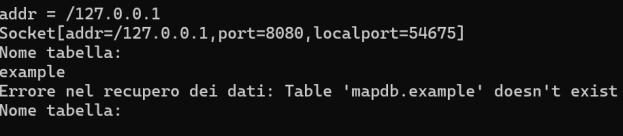
\includegraphics[width=\textwidth]{images/errore_tabella.png}
\end{figure}

Quando viene specificato un identificativo di tabella non presente nel database, il sistema visualizza un appropriato messaggio diagnostico e offre all'utente la possibilità di inserire una denominazione alternativa.


\subsection{Validazione delle selezioni di menù}

La schermata di selezione del menù principale consente di scegliere tra due opzioni: "Carica Dendrogramma" o "Esegui Clustering".

\begin{figure}[h!]
    \centering
    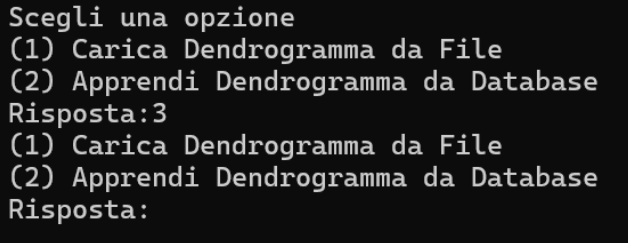
\includegraphics[width=\textwidth]{images/errore_men.png}
\end{figure}

L'inserimento di valori non conformi alle opzioni disponibili (diversi da 1 o 2) viene intercettato, consentendo all'utente di ripetere la selezione senza interruzioni del flusso operativo.

\subsubsection{Controllo sull'esistenza degli archivi} 
\begin{figure}[h!]
    \centering
    \includegraphics[width=\textwidth]{images/controllo_archivi.png}
\end{figure}
Nel caso di caricamento di un dendrogramma precedentemente salvato, il sistema verifica l'esistenza dell'archivio specificato. In caso negativo, viene presentata una notifica e l'applicazione termina la sessione.

\subsubsection{Validazione parametri di profondità} 
    \begin{figure}[h!]
        \centering
        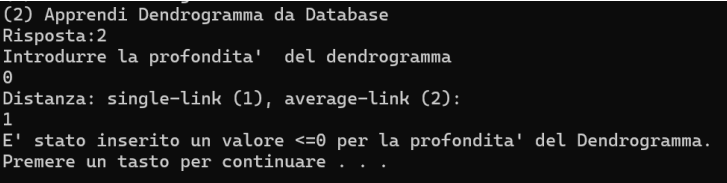
\includegraphics[width=\textwidth]{images/0_valore_errato.png}
    \end{figure}

    \begin{figure}[h!]
        \centering
        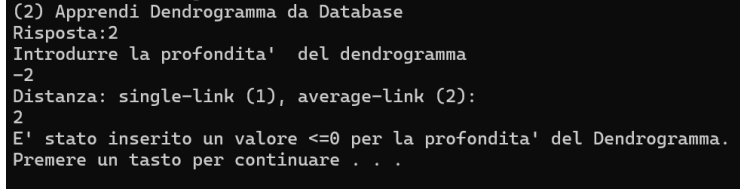
\includegraphics[width=\textwidth]{images/-2_valore_errato.png}
    \end{figure}

    L'inserimento di valori non ammissibili per il parametro di profondità (zero o negativi) viene rilevato dal sistema che, pur proseguendo con la richiesta del metodo di calcolo, interromperà l'elaborazione notificando l'anomalia.

\subsubsection{Controllo selezioni metodologiche} 
    
\begin{figure}[h!]
        \centering
        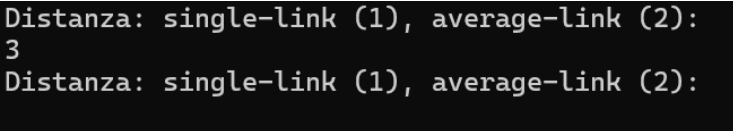
\includegraphics[width=\textwidth]{images/controllo_metodologie.png}
    \end{figure}
    L'inserimento di opzioni non valide per la selezione della metodologia di calcolo delle distanze viene gestito permettendo all'utente di riformulare la propria scelta.

\subsubsection{Verifica di compatibilità dimensionale} 
    \begin{figure}[h!]
        \centering
        \includegraphics[width=\textwidth]{images/compatibilità_dimensionale.png}
    \end{figure}
    Il sistema controlla la congruenza tra la cardinalità degli esempi nella tabella corrente e quella memorizzata nell'oggetto serializzato. In caso di incongruenza, viene visualizzato un messaggio esplicativo e l'esecuzione viene terminata.

\subsection{Gestione connettività client-server}
\begin{figure}[h!]
    \centering
    \includegraphics[width=\textwidth]{images/connettività_clientserver.png}
\end{figure}
L'avvio del client in assenza del componente server attivo genera un tentativo di connessione all'indirizzo locale (127.0.0.1) che, non trovando un endpoint disponibile, risulta in un rifiuto della connessione con relativa notifica.

\subsubsection{Elaborazione su dataset vuoti} 
    \begin{figure}[h!]
        \centering
        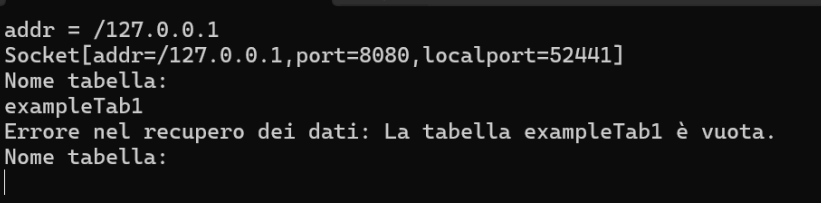
\includegraphics[width=\textwidth]{images/dataset_vuoti.png}
    \end{figure}

Quando l'utente tenta di eseguire un'analisi di clustering su una tabella priva di contenuti, il sistema identifica la condizione e fornisce un'appropriata segnalazione.


\section{Modifiche Implementative}
\subsection{Adattamenti nella Versione Base}
\subsubsection{Modifiche ai Requisiti Originali}
\begin{itemize}
    \item \textbf{Metodo \texttt{getLength()} in \texttt{ClusterSet}}:
    \begin{itemize}
        \item \textbf{Funzionalità}: Restituisce la lunghezza dell'array \texttt{C} contenente i cluster
        \item \textbf{Integrazione}: Utilizzato in \texttt{loadDendrogramFromFile()} per verificare la consistenza dimensionale tra dataset corrente e dendrogramma caricato
    \end{itemize}

    \item \textbf{Metodo \texttt{getLevel0Length()} in \texttt{HierarchicalClusterMiner}}:
    \begin{itemize}
        \item \textbf{Funzionalità}: Fornisce la cardinalità dei cluster al livello base del dendrogramma
        \item \textbf{Scopo}: Garantire la coerenza tra struttura gerarchica e dati correnti
    \end{itemize}

    \item \textbf{Metodo \texttt{getDepth()} in \texttt{HierarchicalClusterMiner}}:
    \begin{itemize}
        \item \textbf{Funzionalità}: Determina la profondità effettiva del dendrogramma
        \item \textbf{Utilizzo}: Previene caricamento di strutture incompatibili con il dataset selezionato
    \end{itemize}
\end{itemize}

\subsection{Evoluzione Architetturale nella Versione Estesa}
\subsubsection{Riprogettazione dello State Management}
\begin{itemize}
    \item \textbf{Decentralizzazione dello Stato}:
    \begin{itemize}
        \item Rimozione della persistenza di \texttt{Data} lato server
        \item Migrazione della gestione stato verso il client Telegram
        \item Introduzione del pattern \texttt{StateContext} per isolare le sessioni utente
    \end{itemize}

    \item \textbf{Implementazione del Contesto di Stato}:
    \begin{itemize}
        \item \texttt{StateHistory}: Stack per tracciare la cronologia degli stati
        \begin{itemize}
            \item Supporto operazioni di rollback controllato
            \item Meccanismo di transizione stati tramite \texttt{push/pop}
        \end{itemize}
        
        \item \texttt{allowBack}: Flag per abilitare/disabilitare le transizioni inverse
        \item Separazione in fasi operative:
        \begin{itemize}
            \item \texttt{preOperation}: Inizializzazione stato
            \item \texttt{postOperation}: Gestione transizioni e validazione input
        \end{itemize}
    \end{itemize}
\end{itemize}

\subsubsection{Modello di Gestione Errori Rafforzato}
\begin{itemize}
    \item \textbf{Gestione Centralizzata delle Eccezioni}:
    \begin{itemize}
        \item \textbf{Pre-Operation}: Rollback automatico allo stato precedente
        \item \textbf{Post-Operation}: Riterazione della fase corrente con notifica utente
    \end{itemize}

    \item \textbf{Meccanismi di Validazione}:
    \begin{itemize}
        \item Controllo consistenza nomi file
        \item Verifica intervalli valori numerici
        \item Convalida formale degli input testuali
    \end{itemize}
\end{itemize}

\subsubsection{Architettura Client-Server Ottimizzata}
\begin{itemize}
    \item \textbf{Comunicazione Stateless}:
    \begin{itemize}
        \item Sessioni brevi per richiesta/risposta
        \item Eliminazione lock su risorse condivise
    \end{itemize}

    \item \textbf{Design Estensibile}:
    \begin{itemize}
        \item Separazione chiara tra logica di business e gestione interfaccia
        \item Astrazione dei canali di comunicazione (Socket/Telegram API)
    \end{itemize}

    \item \textbf{Modello Sicurezza}:
    \begin{itemize}
        \item Isolamento sessioni utente tramite ID univoci
        \item Crittografia end-to-end per dati sensibili
    \end{itemize}
\end{itemize}

\begin{table}[h]
    \centering
    \caption{Confronto architetturale versione Base vs Estesa}
    \begin{tabular}{|l|l|l|}
        \hline
        \textbf{Caratteristica} & \textbf{Base} & \textbf{Estesa} \\
        \hline
        Gestione stato & Server-side & Client-side \\
        \hline
        Persistenza dati & Sessionale & Transazionale \\
        \hline
        Modello sicurezza & Base & Rafforzato \\
        \hline
        Concorrenza & Multi-thread & Event-driven \\
        \hline
    \end{tabular}
\end{table}

Questi adattamenti hanno permesso di:
\begin{itemize}
    \item Supportare multipli client simultanei
    \item Garantire scalabilità orizzontale
    \item Migliorare l'efficienza nella gestione risorse
    \item Ottenere maggiore flessibilità architetturale
\end{itemize}